\documentclass[tikz,border=10pt]{standalone}
\usepackage{amsmath}
\usetikzlibrary{angles,quotes,calc}
\begin{document}
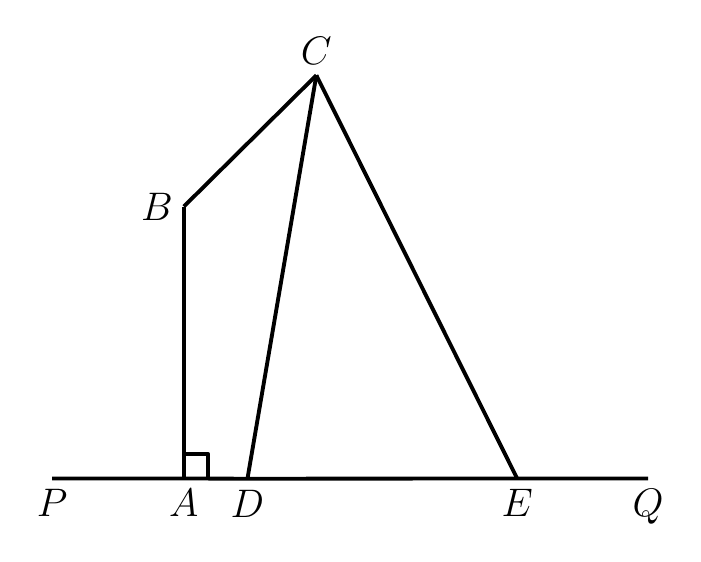
\begin{tikzpicture}[line join=round, line width=1.4pt]
\coordinate (A) at (-2.130,-2.490);
\coordinate (B) at (-2.130,0.963);
\coordinate (C) at (-0.447,2.630);
\coordinate (D) at (-1.322,-2.494);
\coordinate (P) at (-3.802,-2.490);
\coordinate (Q) at (3.766,-2.490);



\coordinate (E) at (2.103,-2.490);


\draw (P) -- (A) -- (D) -- (E) -- (Q);


\draw (A) -- (B);
\draw (B) -- (C);
\draw (C) -- (D);
\draw (C) -- (E);


\draw pic[draw, angle radius=0.310cm, line width=1.4pt] {right angle=B--A--Q};


\node[below, font=\fontsize{14}{16.8}\selectfont] at (P) {$P$};
\node[below, font=\fontsize{14}{16.8}\selectfont] at (A) {$A$};
\node[below, font=\fontsize{14}{16.8}\selectfont] at (D) {$D$};
\node[below, font=\fontsize{14}{16.8}\selectfont] at (E) {$E$};
\node[below, font=\fontsize{14}{16.8}\selectfont] at (Q) {$Q$};
\node[left, font=\fontsize{14}{16.8}\selectfont] at (B) {$B$};
\node[above, font=\fontsize{14}{16.8}\selectfont] at (C) {$C$};
\end{tikzpicture}
\end{document}